\documentclass[a4paper,12pt,numbered]{article}

\usepackage{mathtools}
\usepackage{amsmath}
\usepackage{soul}
\usepackage{amssymb,amsmath,amsfonts}
\usepackage[utf8]{inputenc}
\usepackage{graphicx}
\usepackage{geometry}
\usepackage{float}
\usepackage[german=quotes]{csquotes}
\usepackage{hyperref}
\usepackage{fancyhdr}
\usepackage{gensymb}
\usepackage{units}
\usepackage{hhline}
\usepackage{color}
\usepackage[export]{adjustbox}
\usepackage[nottoc,numbib]{tocbibind}
\usepackage[square,numbers]{natbib}
\usepackage{titling}
\usepackage{subfloat}
\usepackage{multicol}
\usepackage{caption}
\usepackage{authblk}
\usepackage{graphics}
\usepackage{subcaption}
\usepackage{pdfpages}

\setlength{\parindent}{0pt}

\begin{document}

\section{Neutrinos}

Neutrinos were first postulated by Wolfgang Pauli in 1930 upon discovering that the energy spectrum of electrons in nuclear beta decay of N- and Li-6 nuclei is continuous. As the energy levels of the decay products of a decay into two particles is discrete, this implied that there must have been a third particle, electrically chargeless and at least similarly small relative to the nucleus, like the electron \cite{Pauli_Letter}.
\\ \\
Since then, three generations of neutrinos have been discovered. The first discovery of neutrinos happened in 1956 at the Savannah River Plant \cite{nuebar_discovery}, with the discovery of the electron neutrino ($\nu_e$). Then, in 1962, the muon neutrino ($\nu_\mu$) was discovered at the Brookhaven National Lab \cite{numu_discovery}. The discovery of the last of the three currently known neutrino generations, the tau neutrino ($\nu_\tau$), took place in 2000 by the DONUT experiment at Fermilab \cite{nutau_discovery}. The number of active neutrino species interacting weakly, with masses below that of the Z-boson $N_\nu =2.9840\pm0.0082$ shows agreement with the amount of discovered neutrino generations \cite{neunumber_constraints}.

\subsection{Neutrinos in the Standard Model}

This section briefly goes through the most relevant aspects of the Standard Model for neutrino physics. A more in-depth review of electroweak interactions and neutrinos in the SM is given in \cite{electroweak_lagrangian}.
\\ \\
In the Standard Model (SM) neutrinos are represented as electromagnetically neutral fermion fields that only interact through the weak force. The neutrinos belonging to each neutrino generation can be grouped together with their charged lepton counterparts as doublets $\begin{pmatrix} \nu_e \\ e^- \end{pmatrix}, \begin{pmatrix} \nu_\mu \\ \mu^- \end{pmatrix}, \begin{pmatrix} \nu_\tau \\ \tau^- \end{pmatrix}$ that transform together under the $SU(2)_L$ symmetry of the weak force, where $L$ indicates left-handed chirality  with left/right-handed chirality of a spin 1/2 fermion field $\Psi$ being defined by

\begin{align}
\Psi_{L/R}=\frac{1\mp \gamma^5}{2}\Psi
\end{align}

with $\gamma^5$ being the fifth gamma matrix of the Dirac algebra. Only left-handed particles and right-handed antiparticles are observed to interact weakly. The part of the SM Lagrangian relevant for interactions of fermions through the weak force after symmetry breaking is

\begin{align}
\begin{split}
-\mathcal{L}_{\text{weak, interaction}} &= 
\frac{g}{\sqrt{2}} \left( \bar{\psi}_L \gamma^\mu \psi'_L W^+_\mu + \text{h.c.} \right) \\
&\quad + \frac{g}{\cos \theta_W} \bar{\psi}_L \gamma^\mu 
\left( T_3 - Q \sin^2 \theta_W \right) \psi_L Z_\mu 
\end{split}
\end{align}

where $g$ is the weak coupling constant, $\psi_L$ the left-handed fermion field, $\psi'_L$ the corresponding other fermion field in the weak doublet. $W^+_\mu$, and $Z_\mu$ are the weak boson fields mediating the interaction, and $\theta_W$ is the Weinberg angle. $T_3$ and $Q$ are the weak isospin and the electric charge.
\\ \\
Due to aforementioned properties of neutrinos, their interactions can thus be separated into two terms, one charged current (CC), and one neutral current (NC)

\begin{align}
-\mathcal{L}_{\text{weak, CC}} &= 
\frac{g}{\sqrt{2}} \left( \bar{\nu}_L \gamma^\mu l^-_L W^+_\mu + \text{h.c.} \right) \\
-\mathcal{L}_{\text{weak, NC}} &= \frac{g}{2\cos \theta_W} \bar{\nu}_L \gamma^\mu \nu_L Z_\mu
\end{align}

where $l^-$ is the respective charged lepton corresponding to the neutrino. 
\\ \\
The Yukawa interaction is the method with which fermion masses are generated in the SM, in which the strength of the coupling of the Higgs field to left- and right-handed components of fermion fields, the Yukawa coupling, determines the fermion mass. For charged leptons, this term is

\begin{align}
\mathcal{L}_Y &= - y_l \bar{L}_L \phi l_R + \text{h.c.} 
\end{align}

$y_l$ is the Yukawa coupling to a charged lepton $l$, while $L_L$ is the full weak isospin doublet, $l_R$ being the corresponding right-handed isospin singlet, and $\phi$ the Higgs doublet. 
\\ \\
As neutrinos only interact weakly and because of the chiral nature of the weak interaction, the SM does not include right-handed neutrino fields. As such, the Yukawa interaction, which is responsible for generating the masses of fermions does not generate a neutrino mass term after electroweak symmetry breaking. Thus neutrinos are massless in the SM.

\subsection{Neutrino Oscillations}

The discovery of neutrino oscillations was motivated by the solar neutrino problem, the measured deficiency in the flux of electron neutrinos from the sun observed in experiments such as Homestake \cite{solneu_history}. In 1998, neutrino oscillations were confirmed at the Super-Kamiokande collaboration, which observed the oscillation of neutrinos produced from cosmic rays propagating through the earth \cite{kamiokande_discovery}.
\\ \\
Neutrino oscillations can be explained by introducing neutrino mass eigenstates $\nu_i$, that mix into the weak flavor eigenstates $\nu_\alpha$ via a unitary matrix $U$, the so called  PMNS (Pontecorvo-Maki-Nakagawa-Sakata) matrix. 

\begin{equation}
    |\nu_\alpha\rangle = \sum_{i=1}^{3} U_{\alpha i} |\nu_i\rangle,
\end{equation}

As the PMNS matrix is a 3x3 complex unitary matrix, its general form can be expressed by the multiplication of three real rotation matrices $R_{ij}$ describing two flavor mixing with respective mixing angles $\theta_{ij}$ and an additional complex phase $\delta_{CP}$ that leads to CP violation.

\begin{equation}
    U_{\text{PMNS}} = R_{23}(\theta_{23}) R_{13}(\theta_{13}, \delta_{CP}) R_{12}
\end{equation}

\begin{align}
\begin{split}
    U_{\text{PMNS}} &= 
    \begin{bmatrix}
        1 & 0 & 0 \\
        0 & \cos_{23} & s_{23} \\
        0 & -s_{23} & \cos_{23}
    \end{bmatrix}
    \begin{bmatrix}
        \cos_{13} & 0 & s_{13} e^{-i\delta_{CP}} \\
        0 & 1 & 0 \\
        -s_{13} e^{i\delta_{CP}} & 0 & \cos_{13}
    \end{bmatrix}
    \begin{bmatrix}
        \cos_{12} & s_{12} & 0 \\
        -s_{12} & \cos_{12} & 0 \\
        0 & 0 & 1
    \end{bmatrix}
    \\
    &=
    \begin{bmatrix}
        c_{12} c_{13} & s_{12} \cos_{13} & s_{13} e^{-i\delta_{CP}} \\
        -s_{12} c_{23} - c_{12} s_{23} s_{13} e^{i\delta_{CP}} & 
        c_{12} c_{23} - s_{12} s_{23} s_{13} e^{i\delta_{CP}} & 
        s_{23} c_{13} \\
        s_{12} s_{23} - c_{12} c_{23} s_{13} e^{i\delta_{CP}} & 
        -c_{12} s_{23} - s_{12} c_{23} s_{13} e^{i\delta_{CP}} & 
        c_{23} c_{13}
    \end{bmatrix}
\end{split}
\end{align}

where $c_{ij}=cos\theta_{ij}, s_{ij}=sin\theta_{ij}$. In the vacuum, the propagation of these mass states $\nu_i$ can be calculated with the Schrödinger equation leading to be a plane wave solution

\begin{equation}
    |\nu_i(t)\rangle = e^{-i E_i t} |\nu_i(0)\rangle,
\end{equation}

for a neutrino with an energy $E_i$ and a propagation time $t$. Assuming relativistic neutrinos the energy is approximately $E_i \approx |\vec{p}_i| + m_i^2 / 2E$, the phase difference depends on the mass-squared differences $\Delta m_{ij}^2 = m_i^2 - m_j^2$. The oscillation probability can then be determined to be

\begin{align}
\begin{split}
\langle \nu_\beta | \nu_\alpha (t) \rangle &= \sum_{i=1}^3 \sum_{j=1}^3 U_{\beta j} U_{\alpha i}^* e^{-i \frac{m_i^2 L}{2E}} \langle \nu_j | \nu_i \rangle.
\\
P_{\alpha \to \beta}(t) &= \left[ \langle \nu_\beta | \nu_\alpha (t) \rangle \right[^2
\\
P_{\alpha \to \beta}(t) &= \sum_{i,j} U_{\beta i} U_{\beta j}^* U_{\alpha i}^* U_{\alpha j} e^{-i \frac{\Delta m_{ij}^2 L}{2E}}
\end{split}
\end{align}

where the propagation time $t$ has now been replaced by the corresponding length $L$.
For three neutrino flavors this yields

\begin{align}
P_{\alpha \to \beta} = & \delta_{\alpha\beta} - 4 \sum_{i > j} \Re\left( U_{\beta i} U_{\beta j}^* U_{\alpha i}^* U_{\alpha j} \right) \sin^2\left( \frac{\Delta m_{ij}^2 L}{4E} \right) \nonumber \\
& + 2 \sum_{i > j} \Im\left( U_{\beta i} U_{\beta j}^* U_{\alpha i}^* U_{\alpha j} \right) \sin^2\left( \frac{\Delta m_{ij}^2 L}{2E} \right).
\end{align}

where $\delta_{\alpha\beta}$ is the Kronecker-Delta. As the mass splitting between $\Delta m_{21}^2=\mathcal{O}(10^{-5}) \text{ eV}^2$ and $\Delta m_{32}^2=\mathcal{O}(10^{-3}) \text{ eV}^2$ differs by orders of magnitude, a two flavor approximation can sometimes be accurate enough. In that case equation (11) simplifies to

\begin{equation}
P(\nu_\alpha \to \nu_\beta) \approx \sin^2 2\theta \sin^2 \left(\frac{\Delta m^2 L}{4E}\right)
\end{equation}

As equation (12) demonstrates, the oscillation probability is determined by the mixing angles $\Theta$, mass splitting $\Delta m^2$ as well as the length traveled by the neutrino $L$, and the neutrino energy $E$. 

\subsection{Neutrino Production}

Neutrinos from different sources provide opportunities to probe the parameters of the three-flavor neutrino oscillation model in different regimes due to the respective source's energies $E$, baseline lengths $L$, and production mechanisms.
\\
In the following, the different types of sources relevant for the study of neutrino oscillations and production mechanisms will be discussed with particular emphasis on the atmospheric neutrinos relevant for this work. The information included in this section is extracted from chapter 14.6 in \cite{entire_pdg}.

\subsubsection{Solar Neutrinos}

Solar neutrinos are produced in the nuclear fusion processes in the sun, primarily through the $pp$ chain and the CNO cycle. These processes result in the production of electron neutrinos with an average energy below $1 \text{MeV}$.
\\ \\
As such, solar neutrino oscillations can be used to probe the 
$\Delta m^2_{21}$, which dominate at the low energies characteristic of solar neutrinos. The oscillations are further enhanced by the Mikheyev-Smirnov-Wolfenstein (MSW) effect, due to matter interactions in the Sun, making solar neutrinos a powerful probe of $\theta_{12}$.

\subsubsection{Reactor Neutrinos}

Reactor neutrinos are produced via beta decay of neutron-rich fission products in nuclear reactors, primarily as $\bar{\nu}_e$. Reactor experiments at short baselines focus on $\nu_e$ disappearance, which is strongly governed by the mixing angle $\theta_{13}$ and the mass-squared difference $\Delta m^2_{32}$. The precise control over reactor neutrino flux and detection baselines allows for high-precision measurements of these parameters.

\subsubsection{Accelerator Neutrinos}

Accelerator neutrinos are generated by colliding high-energy protons into a target, producing pions and kaons that decay into neutrinos. These neutrinos allow precise control of energy and baseline, enabling the study of all three mixing angles ($\theta_{12}$, $\theta_{13}$, $\theta_{23}$), the mass-squared difference $\Delta m^2_{32}$, and the CP-violating phase $\delta_{\text{CP}}$. Long-baseline accelerator experiments, in particular, provide direct sensitivity to $\delta_{\text{CP}}$ by comparing neutrino and antineutrino oscillations. Together, these sources provide complementary information, enabling a comprehensive exploration of the three-flavor neutrino model.

\subsubsection{Atmospheric Neutrinos}

Atmospheric neutrinos are produced when high-energy cosmic rays, primarily protons, collide with nuclei in Earth’s atmosphere. These interactions generate cascades of secondary particles, including pions and kaons, which decay into muons and neutrinos. For example, a positively charged pion decays via $\pi^+ \to \mu^+ + \nu_\mu$, and the muon subsequently decays as $\mu^+ \to e^+ + \nu_e + \bar{\nu}_\mu$. This chain produces a mixture of muon neutrinos ($\nu_\mu$) and electron neutrinos ($\nu_e$), with $\nu_\mu$ dominating by approximately a factor of two due to the decay kinematics.

Atmospheric neutrinos cover a wide range of energies, from hundreds of MeV to several TeV, and travel along diverse baselines, from a few kilometers (horizontal neutrinos) to over 12,000 kilometers (vertically upward neutrinos passing through Earth's core). This diversity makes atmospheric neutrinos a powerful tool to study neutrino oscillations across multiple scales. The long baselines allow the measurement of oscillations driven by the atmospheric mass-squared difference, $\Delta m^2_{32}$, and the mixing angle $\theta_{23}$. At lower energies, oscillations are also sensitive to subdominant effects from the solar parameters, $\Delta m^2_{21}$ and $\theta_{12}$.

One key feature of atmospheric neutrino studies is their sensitivity to the neutrino mass ordering (normal or inverted). As neutrinos travel through Earth's dense matter, they experience the Mikheyev-Smirnov-Wolfenstein (MSW) effect, which alters the oscillation probabilities differently for neutrinos and antineutrinos depending on the mass hierarchy. By measuring differences in the oscillation patterns of upward-going neutrinos and antineutrinos, experiments like Super-Kamiokande, IceCube, and KM3NeT can probe the mass ordering. Additionally, these matter effects are sensitive to the octant of $\theta_{23}$—whether it is less than or greater than $45^\circ$—providing further constraints on this parameter.

High-energy atmospheric neutrinos also allow tests of exotic phenomena beyond the standard three-flavor model. For instance, deviations from expected oscillation patterns at TeV energies could signal new physics, such as sterile neutrinos, non-standard interactions, or violations of Lorentz invariance. The large event samples and energy-angular coverage in experiments like IceCube make atmospheric neutrinos a unique probe of such effects. Together, atmospheric neutrino studies provide vital insights into neutrino mixing, the mass ordering, and the possibility of physics beyond the standard model.


\begin{table}[h!]
\centering
\scalebox{0.7}{
\begin{tabular}{|c|c|c|c|}
\hline
\textbf{Neutrino Type} & \textbf{Primary Sensitivities} & \textbf{Parameter Ranges} \\ \hline
Solar (\(\nu_e\))& \(\Delta m_{21}^2, \theta_{12}\) & \( \Delta m_{21}^2 \sim 7.4 \times 10^{-5} \, \text{eV}^2 \), \( \sin^2 \theta_{12} \sim 0.3 \) \\ \hline
Atmospheric (\(\nu_\mu, \nu_\tau\))& \(\Delta m_{32}^2, \theta_{23}, \text{Mass Ordering}\) & \( |\Delta m_{32}^2| \sim 2.5 \times 10^{-3} \, \text{eV}^2 \), \( \sin^2 \theta_{23} \sim 0.5 \) \\ \hline
Reactor (\(\bar{\nu}_e\))& \(\Delta m_{21}^2, \theta_{12}, \theta_{13}\) & \( \sin^2 2\theta_{13} \sim 0.09 \), \( \Delta m_{21}^2 \sim 7.4 \times 10^{-5} \, \text{eV}^2 \) \\ \hline
Accelerator (\(\nu_\mu \to \nu_e\))& \(\delta_{\text{CP}}, \theta_{13}, \text{Mass Ordering}\) & \( \delta_{\text{CP}} \sim [-\pi, \pi] \), \( \sin^2 2\theta_{13} \sim 0.09 \) \\ \hline
Cosmological (\(\nu\)) & Total Mass & \( \Sigma m_\nu \lesssim 0.12 \, \text{eV} \) \\ \hline
\end{tabular}
}
\caption{Types of Neutrinos and Their Oscillation Sensitivities}

\end{table}

\subsection{Neutrino Oscillations in Matter}

While the equations so far derived in the chapter 1.2 for the oscillation probability of neutrino flavors hold in vacuum, the presence of electrons, protons and neutrons in stable matter, allows the interaction of propagating neutrinos through charged- and neutral current interactions.
\\
Depending on the energy range

\subsubsection{The MSW Effect}

The Mikheyev-Smirnov-Wolfenstein (MSW) effect describes how the addition effective potentials alter neutrino oscillations due to the presence of matter. This effect is particularly relevant for solar and atmospheric neutrino oscillations.

In matter, neutrinos interact with electrons, and this interaction modifies the neutrino's effective potential. The presence of matter leads to a resonance condition where the neutrino flavor conversion probability can be maximized. The MSW effect plays a significant role in the solar neutrino problem and was crucial in explaining the deficit in the observed electron neutrinos.

The MSW effect modifies the effective Hamiltonian for neutrinos in matter, adding a matter potential term \( V_e \), which affects the oscillation probabilities:

\[
P(\nu_e \to \nu_\alpha) = \sin^2 2\theta_{\text{eff}} \sin^2 \left(\frac{\Delta m^2 L}{4E}\right)
\]

where \( \theta_{\text{eff}} \) is the effective mixing angle in the presence of matter, which depends on the electron density.

The sign of the matter potential is flipped depending on whether one considers neutrinos or antineutrinos. As such, the MSW effect affects the oscillation probability of neutrinos and antineutrinos differently.


\subsubsection{Neutrino Mass Ordering}

The consequence of equation (11) and (12) is that the measurement of neutrino oscillations gives us access to the parameters of the PMNS matrix as well as the mass splitting but not the absolute mass.
\\ 
There are two possible cases for the mass ordering to match our observations: normal ordering (NO), in which $m_1 < m_2 < m_3$, and inverted ordering (IO) $m_3 < m_1 < m_2$. 

\begin{figure}[H]
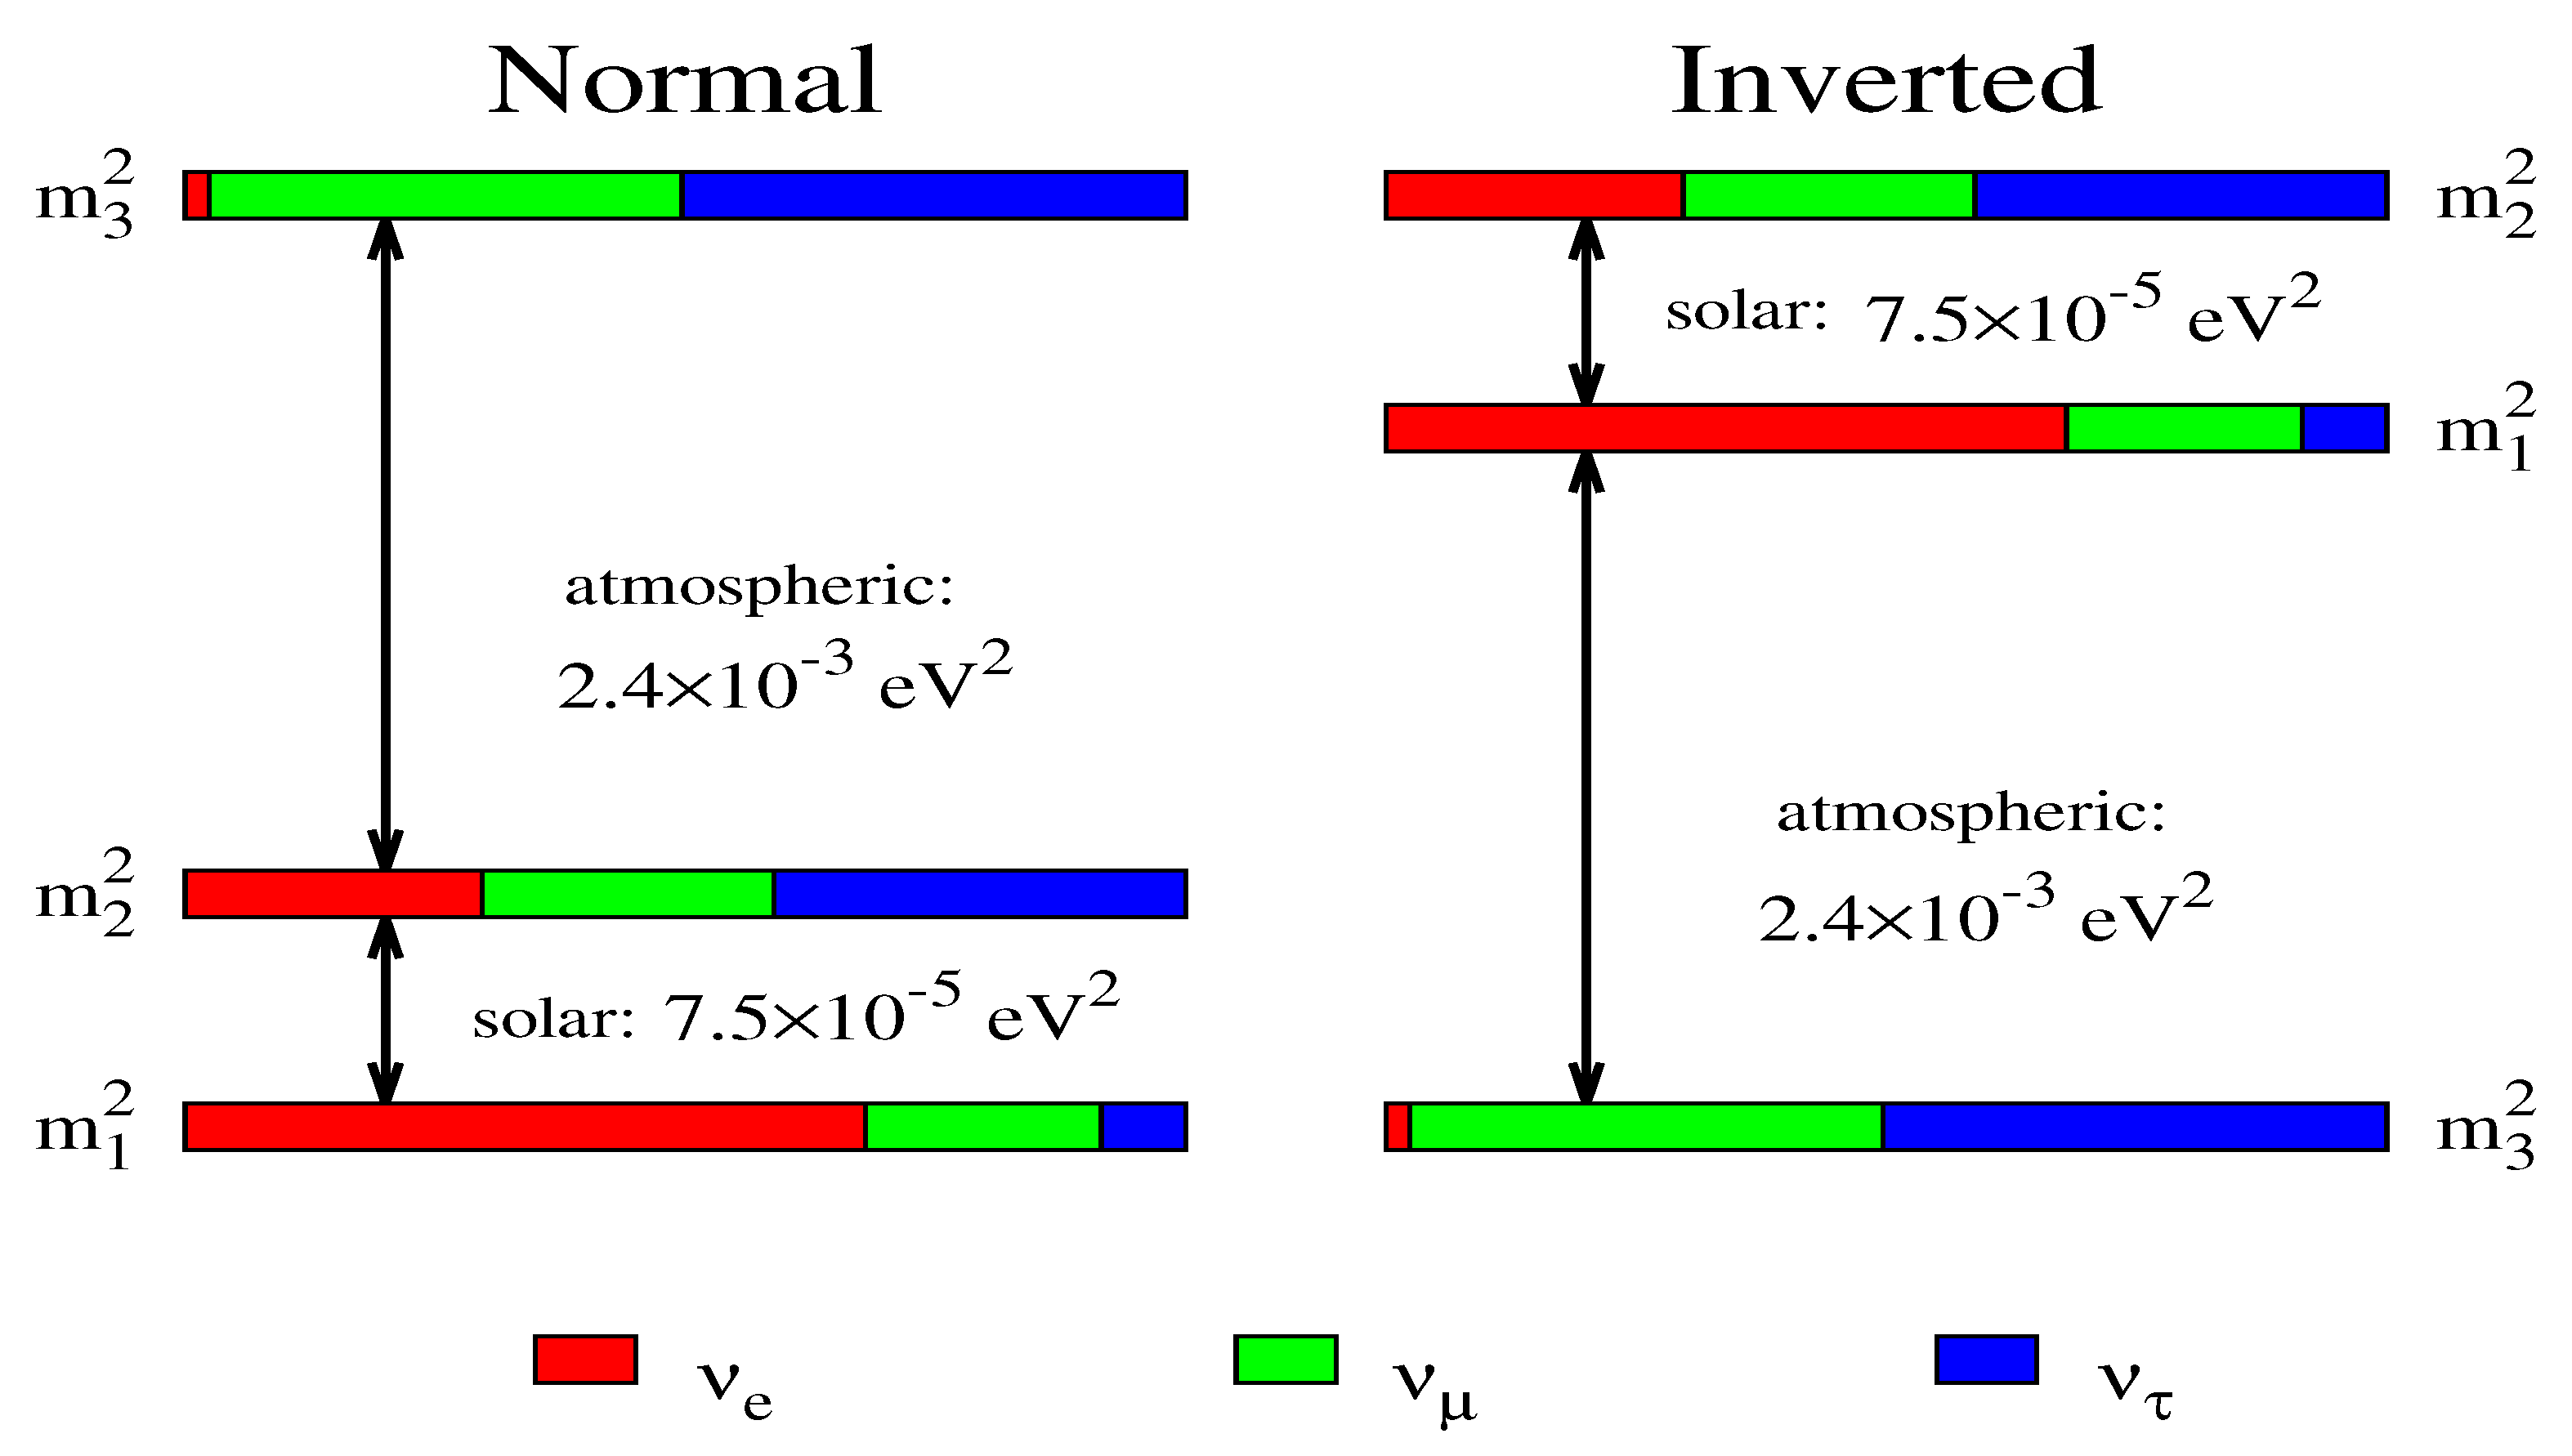
\includegraphics[width=\textwidth]{Neutrino_Figures/nmo.png}
\caption{Composition of neutrino mass eigenstates $m_i$ in terms of the flavor eigenstates for normal and inverted ordering, extracted from \cite{nmo_image_source}}
\end{figure}

While the question of the neutrino mass ordering remains open, significant results for the answer of this question are expected in the near future \cite{future_nmo_sensitivity}. As an investigation of the mass ordering would well be worth its own analysis and surpass the scope of this work, only the case of normal ordering will be considered in this work.

\subsubsection{Oscillation Anomalies}
Over the years, several experiments have reported anomalies in neutrino oscillation data that suggest the presence of new physics. The LSND experiment observed an excess of electron antineutrinos in a muon neutrino beam, which could imply the existence of a sterile neutrino, a hypothesized fourth type of neutrino. Similarly, the reactor neutrino anomaly reported a deficit in the expected electron antineutrino flux, which might also point to the existence of sterile neutrinos or a systematic error in reactor neutrino measurements.

These anomalies have led to the proposal of new neutrino states (e.g., sterile neutrinos) that could account for these discrepancies. However, these results remain controversial, and further experiments are needed to confirm or refute the presence of sterile neutrinos.

\subsubsection{Atmospheric Neutrinos and Production}
Atmospheric neutrinos are produced when high-energy cosmic rays interact with the Earth's atmosphere, primarily producing pions and kaons, which decay into muons and neutrinos:

\[
\pi^\pm \to \mu^\pm + \nu_\mu \quad \text{(decay of pions)}
\]

The Super-Kamiokande experiment observed the oscillation of muon neutrinos produced in the atmosphere, showing that the number of detected muon neutrinos was lower than expected. This deficit provided direct evidence of neutrino oscillations, as the muon neutrinos were oscillating into tau neutrinos, which are more difficult to detect.

Atmospheric neutrinos are an essential tool for testing the neutrino oscillation hypothesis and understanding neutrino properties such as mixing angles and mass squared differences.


The current best-fit values for these parameters are summarized in Table~\ref{tab:neutrino_params}.

\begin{table}[h!]
\centering
\begin{tabular}{|c|c|c|}
\hline
\textbf{Parameter} & \textbf{Value} & \textbf{Reference} \\
\hline
\(\Delta m^2_{21} \, (\text{eV}^2)\) & \(7.53 \times 10^{-5}\) & \cite{Fogli_2012} \\
\(\Delta m^2_{31} \, (\text{eV}^2)\) & \(-2.44 \times 10^{-3}\) & \cite{Fogli_2012} \\
\(\theta_{12}\) (mixing angle) & \(33.48^\circ\) & \cite{Fogli_2012}, \cite{Fukuda_2002} \\
\(\theta_{23}\) (mixing angle) & \(42.0^\circ\) (best fit) & \cite{T2K_2023} \\
\(\theta_{13}\) (mixing angle) & \(8.57^\circ\) & \cite{T2K_2023} \\
\(\delta_{\text{CP}}\) (phase) & \( \text{unknown} \) & \cite{Fogli_2012}, \cite{T2K_2023} \\
\hline
\end{tabular}
\caption{Current best-fit values for neutrino oscillation parameters.}
\end{table}

\subsection{Neutrino Oscillation Anomalies}

The mo

Neutrino oscillation anomalies refer to experimental results that deviate from the expectations of the standard three-flavor neutrino model. These anomalies could indicate new physics, such as sterile neutrinos or exotic interactions, or they might arise from unresolved systematic uncertainties in experimental methods or theoretical predictions. Key anomalies include those observed in the LSND, MiniBooNE, reactor neutrino, and gallium experiments.

\subsubsection{LSND Anomaly}  
The Liquid Scintillator Neutrino Detector (LSND) experiment reported an unexpected excess of $\bar{\nu}_e$ in a beam of $\bar{\nu}_\mu$ neutrinos, with a mass-squared difference ($\Delta m^2$) that cannot be reconciled with solar or atmospheric oscillation scales. This result hinted at the possible existence of sterile neutrinos.

\subsubsection{MiniBooNE Anomaly}  
The MiniBooNE experiment confirmed some of the LSND findings, observing an excess of electron-like events in both neutrino and antineutrino modes at short baselines. These results suggest potential new physics beyond the three-flavor model, with interpretations involving sterile neutrinos or alternative explanations such as unexpected detector or background effects.

\subsubsection{Reactor Antineutrino Anomaly}  
Reactor-based experiments have measured a persistent deficit in the detected $\bar{\nu}_e$ flux compared to theoretical predictions, with the discrepancy potentially explained by oscillations into sterile neutrinos at a mass scale around 1~eV$^2$. Alternatively, uncertainties in predicted reactor antineutrino spectra could be a factor.

\subsubsection{Gallium Anomaly}  
Gallium-based solar neutrino detectors, such as those in the GALLEX and SAGE experiments, observed fewer neutrinos than expected when tested with radioactive sources. This deficit aligns with short-baseline oscillations involving sterile neutrinos, though other explanations are also being investigated.

These anomalies are subjects of intense study, with upcoming experiments and refined models aiming to clarify their nature and potential implications for neutrino physics.


\section{Sterile Neutrinos}

Sterile neutrinos are hypothesized neutrinos that do not interact via the weak force and thus do not participate in the usual SU(2) weak interaction. They are typically proposed in models beyond the Standard Model (BSM) to explain anomalies in neutrino data, such as the LSND and reactor neutrino anomalies. In the 3+1 model, sterile neutrinos are added as a fourth neutrino state, beyond the three active flavors. These sterile neutrinos are assumed to have a mass at the eV2 scale, which can lead to observable effects in neutrino oscillations.

\subsection{The 3+1 Neutrino Model}

The simplest extension of the three-flavor neutrino model involves introducing one additional sterile neutrino \( \nu_s \), resulting in the 3+1 model. In this model, the total number of neutrino mass eigenstates increases to four, and the flavor states are described as a superposition of these four mass eigenstates. The evolution of the flavor states over time is then governed by the standard neutrino oscillation formalism, but with an expanded set of mass eigenstates.

The state of the neutrinos can be written as:

\[
|\nu_\alpha\rangle = \sum_{i=1}^{4} U_{\alpha i} |\nu_i\rangle
\]

where \( \alpha = e, \mu, \tau, s \) represents the flavor states and \( i = 1, 2, 3, 4 \) are the mass eigenstates, including the sterile neutrino. The matrix \( U_{\alpha i} \) is the extended PMNS matrix, now a \( 4 \times 4 \) unitary matrix that describes the mixing of the active and sterile neutrinos. The probability of a neutrino flavor transition is given by:

\[
P(\nu_\alpha \to \nu_\beta) = \sum_{i,j} U_{\alpha i} U_{\beta i}^* U_{\alpha j}^* U_{\beta j} \, e^{-i \Delta m^2_{ij} L / 2E}
\]

where \( \Delta m^2_{ij} = m_i^2 - m_j^2 \) represents the mass squared differences between the mass eigenstates, and \( L \) is the distance traveled by the neutrino.

\subsection{Neutrino Mass Generation}

As mentioned in chapter 1.1, neutrinos have no mass in the SM. 

The mass of sterile neutrinos, specifically those with mass scales around the eV² range, can arise through several mechanisms that extend the Standard Model of particle physics. The two most commonly discussed mechanisms are the **seesaw mechanism** and **radiative corrections**, both of which provide a natural way to introduce sterile neutrinos with non-zero mass. These mechanisms allow for the sterile neutrinos to mix with the active neutrino states and participate in oscillations.

\subsection{Seesaw Mechanism}

The **seesaw mechanism** is the most widely accepted explanation for neutrino mass generation and is particularly relevant for neutrinos with a mass scale much larger than that of the active neutrinos. The seesaw mechanism can be implemented in several ways, including the **type I seesaw** and the **type III seesaw**, both of which involve heavy sterile neutrinos.

- In the type I seesaw, a Majorana mass term is introduced for the right-handed neutrinos (sterile neutrinos) \( N_R \), which do not interact via the weak force. The Lagrangian includes a term of the form:

\[
\mathcal{L} = - \frac{1}{2} M_R \overline{N_R^c} N_R + h.c.
\]

where \( M_R \) is the Majorana mass for the sterile neutrinos. This mass term leads to the mixing between the light active neutrinos and the heavy sterile neutrinos, which can be responsible for the small masses observed for the active neutrinos. The mass of the sterile neutrinos is typically on the order of the electroweak scale or higher, leading to a suppressed active neutrino mass. 

For sterile neutrinos with an eV² mass scale, the Majorana mass term for the sterile neutrinos is tuned to be in the eV range, allowing for a possible contribution to short-baseline neutrino oscillations observed in experiments such as LSND and MiniBooNE \cite{LSND, MiniBooNE}.

\subsection{Radiative Mechanisms}

Another possible mass generation mechanism involves radiative corrections, where neutrino masses are generated through loop-level interactions. In this scenario, sterile neutrinos interact via new physics processes at loop level, leading to small masses. This mechanism can generate mass scales at the eV² level through the introduction of new particles, such as scalar fields or additional gauge bosons, that mediate the interactions between active and sterile neutrinos.

\[
m_\nu \sim \frac{y^2}{16\pi^2} \Lambda
\]

where \( y \) is a coupling constant, and \( \Lambda \) is a new energy scale (possibly on the order of GeV to TeV). While less studied than the seesaw mechanism, radiative corrections provide another avenue for generating the required masses for sterile neutrinos in the eV² range.

\subsection{Sterile Neutrino in the 3+1 Model}

In the 3+1 neutrino model, sterile neutrinos with masses on the order of eV² can influence neutrino oscillation experiments, particularly those searching for oscillation anomalies such as the LSND and reactor neutrino anomalies \cite{LSND, MiniBooNE}. These sterile neutrinos mix with the active neutrino states, leading to the modified oscillation probabilities that have been observed in short-baseline experiments. The eV² scale is particularly relevant in the context of sterile neutrino oscillations, where the mixing parameters and mass squared differences are constrained by current experimental data.


\subsection{The Expanded PMNS Matrix}

In the 3+1 model, the PMNS matrix is extended to include the sterile neutrino \( \nu_s \). This matrix, now \( U_{\alpha i} \), has the form:

\[
U = \begin{pmatrix}
U_{e1} & U_{e2} & U_{e3} & U_{e4} \\
U_{\mu1} & U_{\mu2} & U_{\mu3} & U_{\mu4} \\
U_{\tau1} & U_{\tau2} & U_{\tau3} & U_{\tau4} \\
U_{s1} & U_{s2} & U_{s3} & U_{s4}
\end{pmatrix}
\]

This matrix is a 4x4 unitary matrix, with elements \( U_{\alpha i} \) describing the mixing between the flavor eigenstates (\( \nu_e, \nu_\mu, \nu_\tau, \nu_s \)) and the mass eigenstates. The additional sterile neutrino adds complexity to the matrix, introducing new terms that modify the oscillation probabilities.

The mixing of the sterile neutrino is typically parameterized by introducing additional mixing angles \( \theta_{14}, \theta_{24}, \theta_{34} \) between the active neutrinos and the sterile neutrino. The CP-violating phase for the sterile neutrino also enters the matrix, making the matrix a function of more parameters than in the standard 3-flavor model.

\subsection{Current Constraints on Sterile Neutrinos}

Current experimental constraints on the sterile neutrino sector come from a variety of experiments, including long-baseline oscillation experiments (T2K, NOvA), reactor neutrino experiments (Daya Bay, KamLAND), and short-baseline experiments (LSND, MiniBooNE, and Gallium anomalies). 

- The LSND experiment observed a significant excess of electron neutrino appearance in a muon neutrino beam, which could be interpreted as evidence for sterile neutrinos with a mass squared difference of around 1 eV².
- MiniBooNE, which continued the search for sterile neutrinos, reported results that are consistent with the LSND anomaly but have also been interpreted as requiring additional sterile neutrino states.
- Reactor experiments such as Daya Bay and KamLAND have measured neutrino oscillations with high precision and place stringent limits on the mixing between active and sterile neutrinos, particularly constraining the mixing angle \( \theta_{14} \).

The global fit of data from various experiments suggests that while there is some tension between different results, the mass squared difference for the sterile neutrino is likely to be in the range \( 1 \, \text{eV}^2 \). However, definitive confirmation of sterile neutrinos is still elusive, and the possibility of their existence remains a subject of ongoing research.

\begin{table}[h!]
\centering
\begin{tabular}{|c|c|c|c|}
\hline
\textbf{Parameter} & \textbf{Best Fit} & \textbf{Upper Limit} & \textbf{Experiment/Source} \\
\hline
\(\Delta m^2_{41} \, (\text{eV}^2)\) & \(1.0 \) & \(< 1.5\) & LSND, MiniBooNE, reactor anomalies \cite{LSND, MiniBooNE} \\
\hline
\(\theta_{14}\) (mixing angle) & \( < 0.15 \) & \( 0.12 \) & Daya Bay, IceCube, reactor neutrinos \cite{DayaBay, IceCube} \\
\hline
\(\theta_{24}\) (mixing angle) & \( < 0.18 \) & \( 0.14 \) & T2K, NOvA, short-baseline neutrinos \cite{T2K, NOvA} \\
\hline
\(\theta_{34}\) (mixing angle) & \( < 0.14 \) & \( 0.10 \) & T2K, MINOS, Super-Kamiokande \cite{T2K, MINOS, SuperK} \\
\hline
\(\Delta m^2_{43} \, (\text{eV}^2)\) & \( 1.0 \) & \( < 2.5 \) & Global fits, reactor and long-baseline neutrinos \cite{Fogli_2012, DayaBay} \\
\hline
\(\delta_{\text{CP}}\) (CP-violating phase) & Unknown & Constrained \(\sim [-\pi, \pi]\) & Global fits, T2K, NOvA \cite{T2K_2023, NOvA} \\
\hline
\end{tabular}
\caption{Current best-fit values and constraints on the parameters of a sterile neutrino in the 3+1 model. These limits come from various neutrino experiments, with most constraints focused on mixing angles and mass squared differences.}
\label{tab:sterile_constraints}
\end{table}


\subsection{Sterile Neutrino Oscillations}

Sterile neutrinos can contribute to oscillations in several ways. In the 3+1 model, the appearance of sterile neutrinos results in modified oscillation probabilities, with transitions such as \( \nu_\mu \to \nu_s \) or \( \nu_e \to \nu_s \) becoming possible. These oscillations lead to new features in neutrino spectra and have been investigated in experiments designed to detect flavor transitions.

The oscillation probability for a sterile neutrino is modified by the presence of the additional mixing angles. For instance, in a muon neutrino to sterile neutrino transition, the probability is given by:

\[
P(\nu_\mu \to \nu_s) = \sin^2(2\theta_{34}) \sin^2 \left( \frac{\Delta m^2_{31} L}{4E} \right)
\]

where \( \theta_{34} \) is the mixing angle between the muon neutrino and the sterile neutrino, and \( \Delta m^2_{31} \) is the mass squared difference between the mass eigenstates.

\subsection{Sterile Neutrinos and Matter Effects}

In the presence of matter, such as in the Sun or the Earth, the MSW effect can modify the oscillation probabilities of neutrinos. For active neutrinos, the matter effect causes resonant flavor conversion, where the neutrino flavor oscillates into another flavor at a specific resonance energy. For sterile neutrinos, the MSW effect can also influence the oscillation probabilities, particularly in regions of high electron density, such as in the Sun. 

In the 3+1 model, the matter effects on sterile neutrinos are more complicated, as the sterile neutrino will not interact directly with the matter, but will still influence the oscillations of the active neutrinos. This can lead to modified oscillation patterns, especially in long-baseline experiments where neutrinos pass through the Earth and experience matter effects. For example, in solar neutrino oscillations, the presence of a sterile neutrino can change the effective mixing angle, thus modifying the observed oscillation pattern.

The MSW effect for sterile neutrinos is generally weaker than for active neutrinos, but it can still impact the oscillation probability asymmetry, especially for high-energy neutrinos where the matter potential is significant. In this scenario, the transition from an active to a sterile neutrino may exhibit different oscillation probabilities compared to the predictions in the standard 3-flavor model.


\bibliography{neuReferences}
\bibliographystyle{unsrturl}

\end{document}


